
\hypertarget{menu_help}{}
\section{Help}
\index{help menu}
\index{user guide}
\index{ini file}
\index{recognized words}
\index{about}
\index{user list}
\index{discussion group}

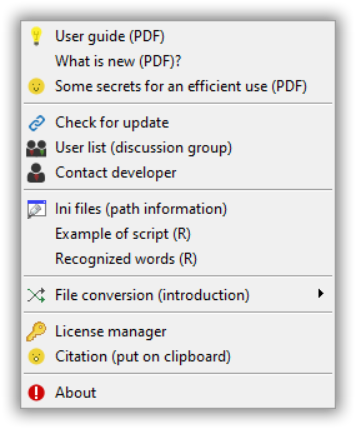
\includegraphics[scale=0.8]{./res/menu_help.png}\\

\begin{scriptsize}
  \begin{tabularx}{\textwidth}{>{\hsize=0.3\hsize}X>{\hsize=0.7\hsize}X}\\
    \hline
    \textbf{Option} & \textbf{Description} \\
    \hline
    User guide (PDF) & Opens the User guide with the PDF viewer default \\
    What is new (PDF)? & Opens the User guide with the PDF viewer default at
     \textit{\href{\#whatisnew}{What is new?}} \\
    Some secrets for an eficient use (PDF) & Opens the User guide with the PDF viewer default at
     \textit{\href{\#secrets}{Some secrets for an eficient use}} \\
    \hdashline[1pt/1pt]
    Check for update & Opens an updater dialog \\
    Licence manager & Opens Licence manager dialog \\
    Contact developer & Opens URL
     \href{https://tinn-r.org/en/contact}
     {Tinn-R Editor - GUI for R Language and Environment contact} \\
    \hdashline[1pt/1pt]
%    User list (discussion group) & Opens URL
%     \href{http://groups.google.com/forum/?fromgroups\#!forum/tinn-r}
%     {Tinn-R Editor - GUI for R Language and Environment user list} \\
    Ini files (path information) & Displays a single dialog with the path information of ini files for Tinn-R \\
    Example of script (R) & Opens the file \textit{Tinn-r\_example of script.r} \\
    Recognized words (R) & Opens the file \textit{Tinn-R\_recognized words.r} \\
    File conversion (introduction) & \textit{\href{\#menu\_help\_main\_fileconversion}{See options ...}} \\
    \hdashline[1pt/1pt]
    Citation (put on clipboard) & Places a text containing the Tinn-R citation in the clipboard \\
    About & Opens the dialog About \\
    \hline
  \end{tabularx}
\end{scriptsize}


\hypertarget{menu_help_main_fileconversion}{}
\subsection{File conversion (introduction)}
\index{help menu!main file conversion}

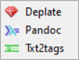
\includegraphics[scale=0.8]{./res/menu_help_conversion.png}\\

\begin{scriptsize}
  \begin{tabularx}{\textwidth}{>{\hsize=0.3\hsize}X>{\hsize=0.7\hsize}X}\\
    \hline
    \textbf{Option} & \textbf{Description} \\
    \hline
    Deplate & Opens the file \textit{deplate\_intro.t2t} \\
    Pandoc & Opens the file \textit{pandoc.markdown} \\
    Txt2tags & Opens the file \textit{txt2tags\_intro.t2t} \\
    \hline
  \end{tabularx}
\end{scriptsize}
